\documentclass{article}
\usepackage[utf8]{inputenc}
\usepackage[letterpaper, margin=1in]{geometry}
\usepackage{graphicx}

\begin{document}

\title{Lab 02}
\label{sec:title}

\section{Prelab}
\label{ssec:subtitle}

\begin{enumerate}
\item
The early late gate method works by taking samples at least 3 points (A, B, C) of the signal.
If C > A, then the samples are traveling uphill. If C < A, then the samples are traveling downhill.
The difference between A and C is proportional to the timing error, and is used in computing
the error. If B is positive, then uphill means sampling happened early and downhill means that
sampling happened late, and visa versa if B is negative. Figure~\ref{fig:earlylate} show examples
of samples being early, late, and on-time.

\begin{figure}[hb]
\centering
\label{fig:earlylate}
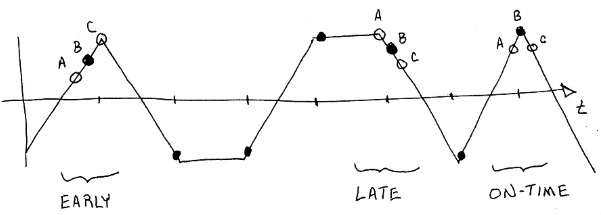
\includegraphics{LateEarlyGate.png}
\caption{Examples of Early-Late Gate}
\end{figure}

\item
Polynomial filter can be used to resample data by

\end{enumerate}

\section{Lab}
\label{ssec:another_subtitle}
\begin{enumerate}
\item[2.]

\begin{figure}[hb]
\centering
\label{fig:ImpulseResRC}
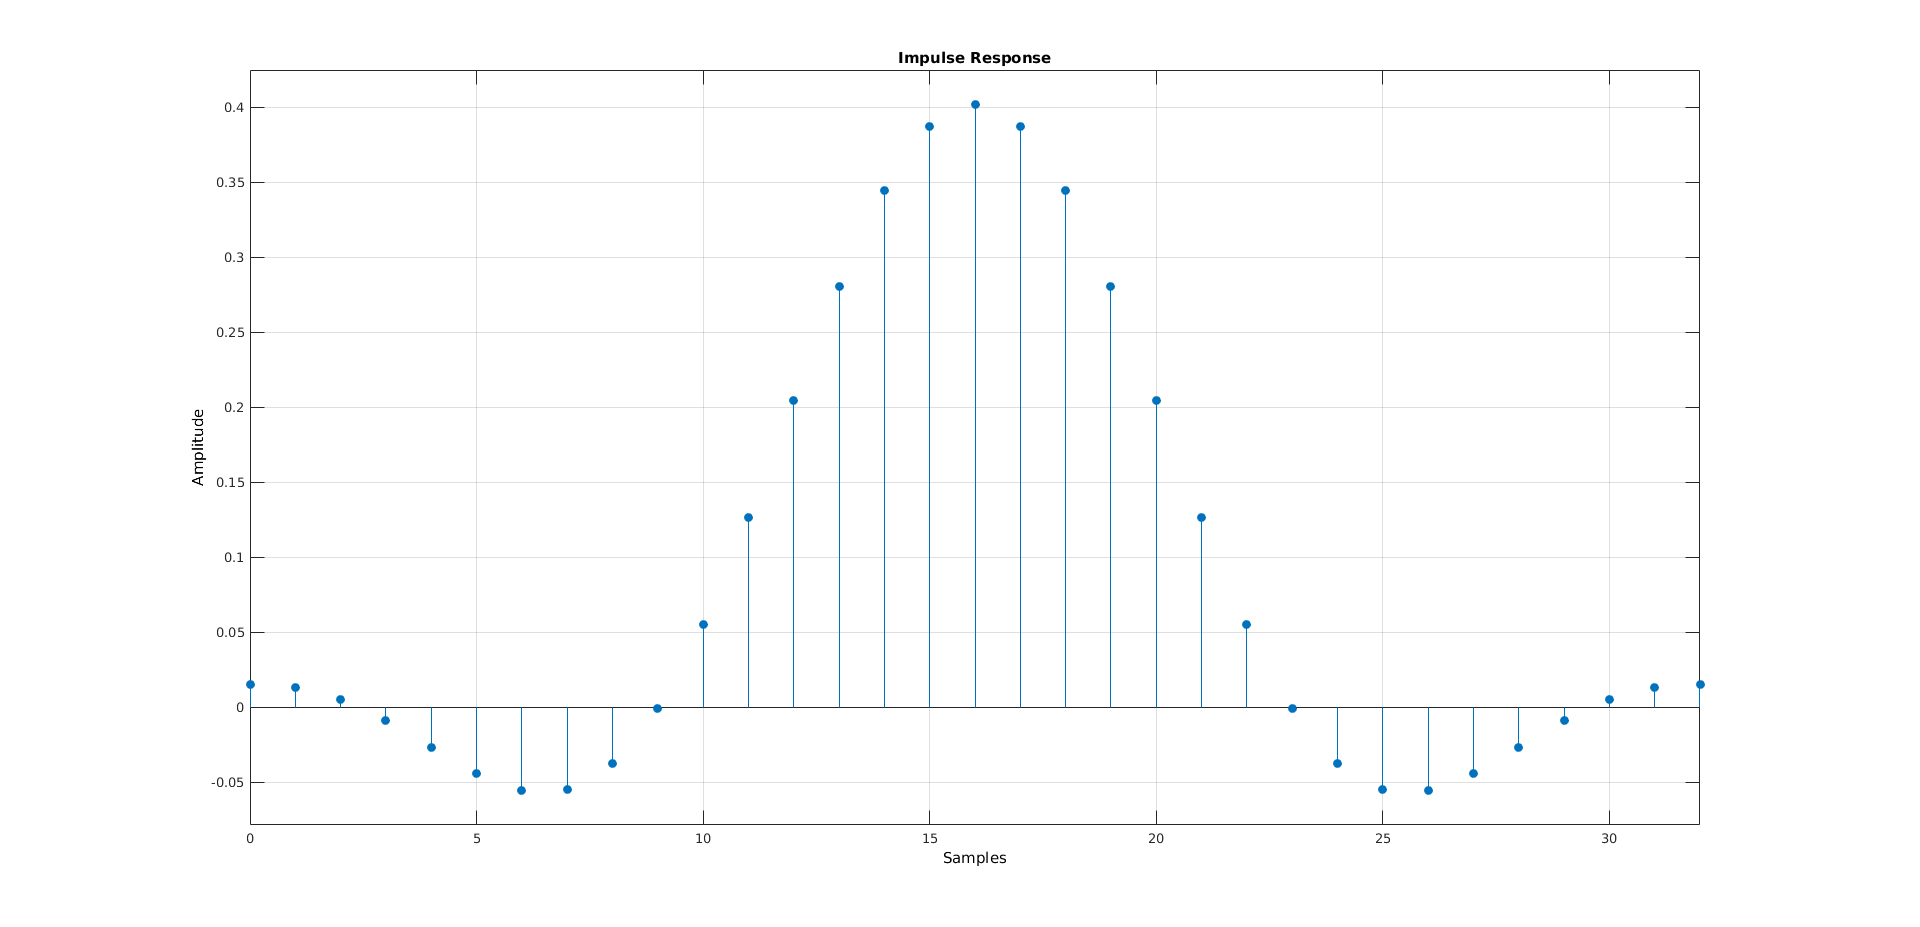
\includegraphics[width=\linewidth]{ImpulseResRC.png}
\caption{Impulse Response of Raised Cosine Function}
\end{figure}

\end{enumerate}

\end{document}